\section{Complex\_\-2D.h File Reference}
\label{Complex__2D_8h}\index{Complex_2D.h@{Complex\_\-2D.h}}
{\tt \#include $<$math.h$>$}\par
{\tt \#include $<$fftw3.h$>$}\par
{\tt \#include $<$Double\_\-2D.h$>$}\par


This graph shows which files directly or indirectly include this file:\begin{figure}[H]
\begin{center}
\leavevmode
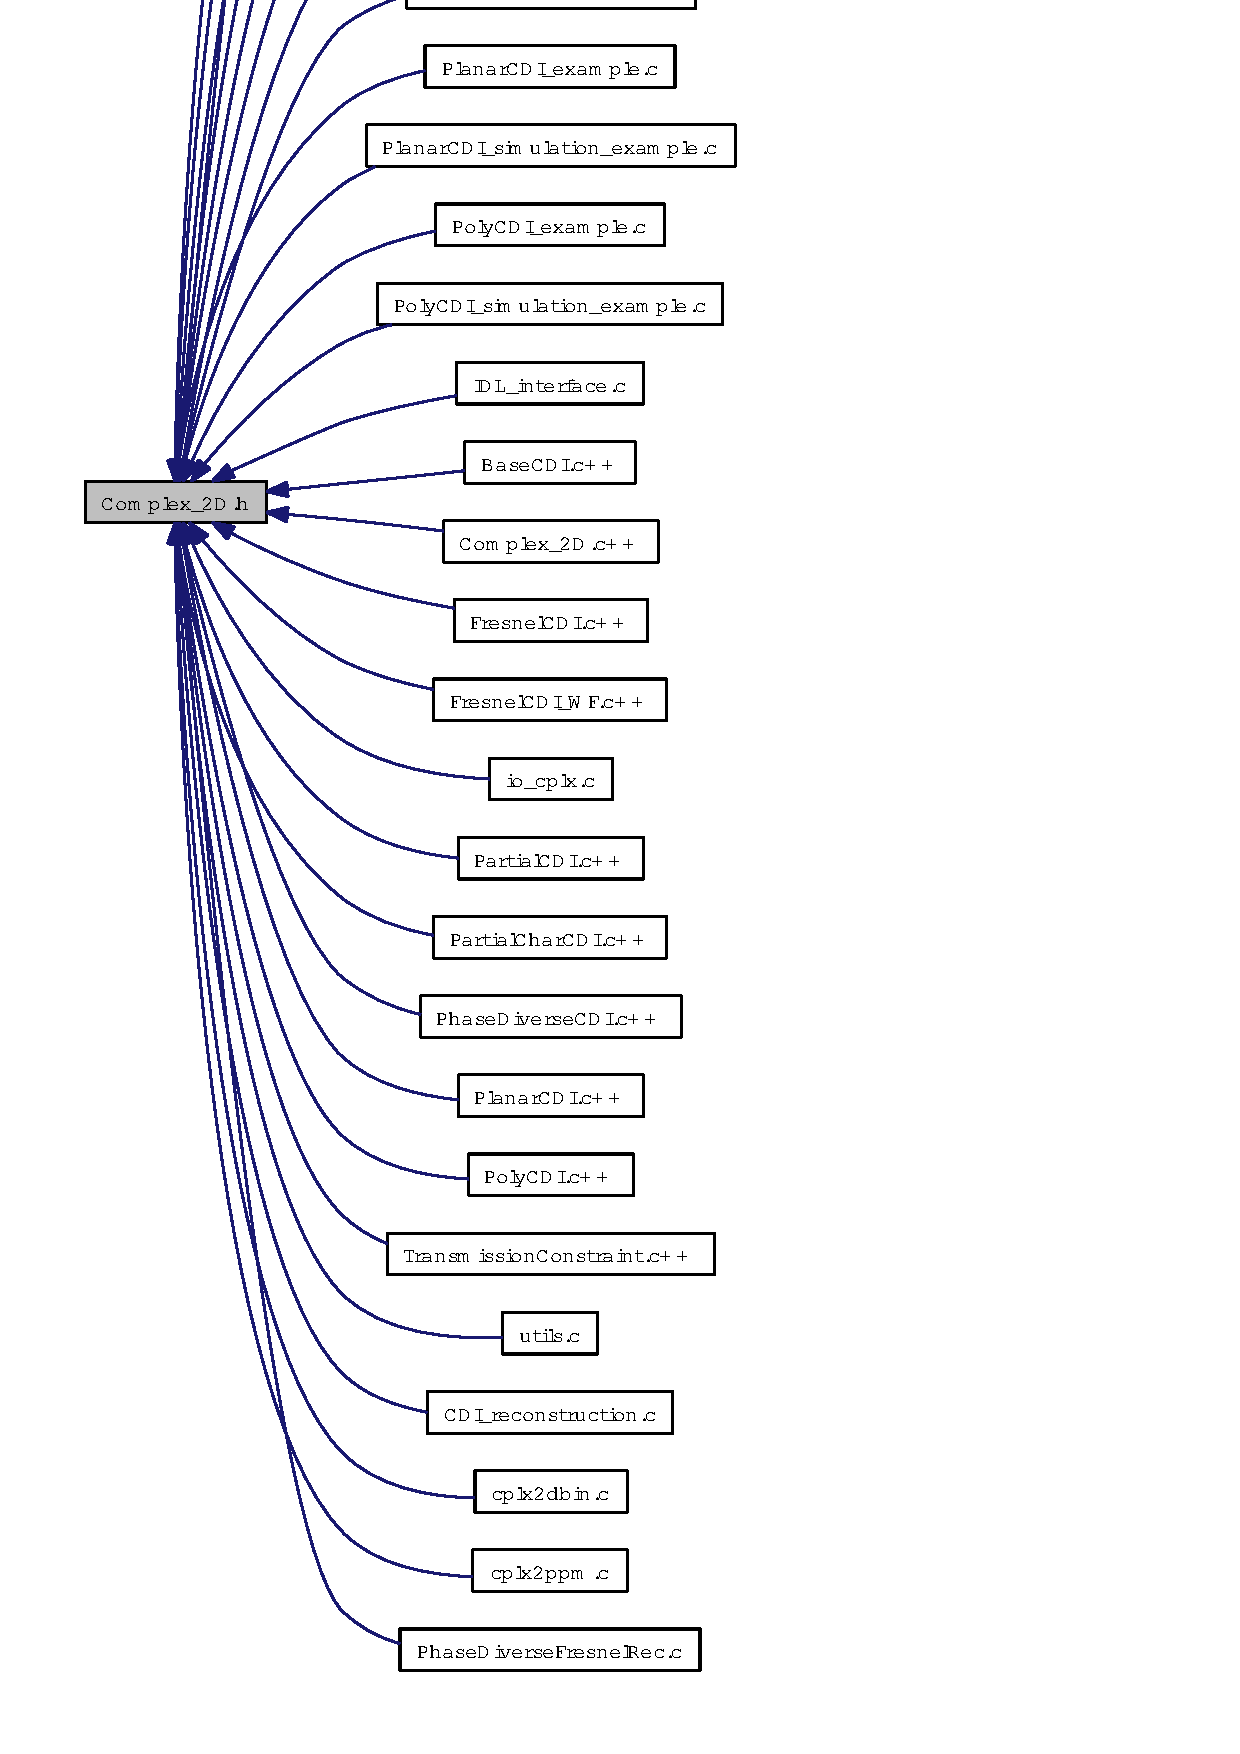
\includegraphics[width=184pt]{Complex__2D_8h__dep__incl}
\end{center}
\end{figure}
\subsection*{Data Structures}
\begin{CompactItemize}
\item 
class \bf{Complex\_\-2D}
\begin{CompactList}\small\item\em A 2-dimensional array of complex numbers. \item\end{CompactList}\end{CompactItemize}
\subsection*{Defines}
\begin{CompactItemize}
\item 
\#define \bf{FAILURE}~0
\item 
\#define \bf{SUCCESS}~1
\item 
\#define \bf{REAL}~0
\item 
\#define \bf{IMAG}~1
\item 
\#define \bf{MAG}~2
\item 
\#define \bf{PHASE}~3
\item 
\#define \bf{MAG\_\-SQ}~4
\end{CompactItemize}


\subsection{Detailed Description}


Definition in file \bf{Complex\_\-2D.h}.

\subsection{Define Documentation}
\index{Complex_2D.h@{Complex\_\-2D.h}!FAILURE@{FAILURE}}
\index{FAILURE@{FAILURE}!Complex_2D.h@{Complex\_\-2D.h}}
\subsubsection{\setlength{\rightskip}{0pt plus 5cm}\#define FAILURE~0}\label{Complex__2D_8h_bbb472742c04f963c42893209fc25a99}


the function failed 

Definition at line 32 of file Complex\_\-2D.h.\index{Complex_2D.h@{Complex\_\-2D.h}!SUCCESS@{SUCCESS}}
\index{SUCCESS@{SUCCESS}!Complex_2D.h@{Complex\_\-2D.h}}
\subsubsection{\setlength{\rightskip}{0pt plus 5cm}\#define SUCCESS~1}\label{Complex__2D_8h_f5b270a7f68ce2ff7f4ddeb8dfe35550}


the function finished successfully 

Definition at line 35 of file Complex\_\-2D.h.\index{Complex_2D.h@{Complex\_\-2D.h}!REAL@{REAL}}
\index{REAL@{REAL}!Complex_2D.h@{Complex\_\-2D.h}}
\subsubsection{\setlength{\rightskip}{0pt plus 5cm}\#define REAL~0}\label{Complex__2D_8h_73aacd4e78f040415d71422e3c30baf5}


real component 

Definition at line 38 of file Complex\_\-2D.h.\index{Complex_2D.h@{Complex\_\-2D.h}!IMAG@{IMAG}}
\index{IMAG@{IMAG}!Complex_2D.h@{Complex\_\-2D.h}}
\subsubsection{\setlength{\rightskip}{0pt plus 5cm}\#define IMAG~1}\label{Complex__2D_8h_24b8c551ca667dbb67122d694fb9b2e8}


imaginary component 

Definition at line 41 of file Complex\_\-2D.h.\index{Complex_2D.h@{Complex\_\-2D.h}!MAG@{MAG}}
\index{MAG@{MAG}!Complex_2D.h@{Complex\_\-2D.h}}
\subsubsection{\setlength{\rightskip}{0pt plus 5cm}\#define MAG~2}\label{Complex__2D_8h_c58faf2647b4a054cdacba0191bd5c99}


magnitude 

Definition at line 44 of file Complex\_\-2D.h.\index{Complex_2D.h@{Complex\_\-2D.h}!PHASE@{PHASE}}
\index{PHASE@{PHASE}!Complex_2D.h@{Complex\_\-2D.h}}
\subsubsection{\setlength{\rightskip}{0pt plus 5cm}\#define PHASE~3}\label{Complex__2D_8h_c0e9e3be78e0764ea150d8fb130bd033}


phase 

Definition at line 47 of file Complex\_\-2D.h.\index{Complex_2D.h@{Complex\_\-2D.h}!MAG_SQ@{MAG\_\-SQ}}
\index{MAG_SQ@{MAG\_\-SQ}!Complex_2D.h@{Complex\_\-2D.h}}
\subsubsection{\setlength{\rightskip}{0pt plus 5cm}\#define MAG\_\-SQ~4}\label{Complex__2D_8h_3a8bc81c6212a1fa55d017066cb1af7d}


magnitudes squared 

Definition at line 50 of file Complex\_\-2D.h.